% Bao cao Bai thuc hanh 04 - TurtleBot 4 Simulation co ban
% Bien dich: xelatex report.tex  (chay 2 lan)   hoac   lualatex report.tex
\documentclass[11pt,a4paper]{article}
\usepackage[a4paper,margin=2.3cm]{geometry}
\usepackage{fontspec}
\setmainfont{Liberation Serif}
\setsansfont{Liberation Sans}
\setmonofont{DejaVu Sans Mono}[Scale=0.82]
\usepackage{amsmath}
\usepackage{graphicx,xcolor,booktabs,float,caption,subcaption,enumitem,longtable,listings}
\usepackage{tikz}
\usetikzlibrary{positioning,arrows.meta,fit,backgrounds}
\usepackage[hidelinks]{hyperref}
\graphicspath{{../figures/}{figures/}}
\setlist{itemsep=2pt,topsep=3pt}
\captionsetup{font=small,labelfont=bf}
\renewcommand{\figurename}{Hình}
\renewcommand{\tablename}{Bảng}
\renewcommand{\contentsname}{Mục lục}
\renewcommand{\abstractname}{Tóm tắt}
\renewcommand{\lstlistingname}{Mã}

\definecolor{codebg}{gray}{0.96}
\definecolor{cmt}{rgb}{0.15,0.45,0.15}
\definecolor{kw}{rgb}{0.1,0.2,0.65}
\lstset{basicstyle=\ttfamily\small,backgroundcolor=\color{codebg},frame=single,
  rulecolor=\color{black!25},breaklines=true,breakatwhitespace=false,columns=fullflexible,
  keepspaces=true,showstringspaces=false,commentstyle=\color{cmt},keywordstyle=\color{kw},
  numbers=left,numberstyle=\tiny\color{gray},xleftmargin=1.6em,framexleftmargin=1.2em,
  aboveskip=6pt,belowskip=4pt,captionpos=b}
\lstdefinelanguage{yaml}{morekeywords={true,false,True,False},sensitive=true,
  morecomment=[l]{\#},morestring=[b]",morestring=[b]'}
\lstdefinelanguage{bash}{morekeywords={source,export,exec,until,do,done,for,in,echo,set,if,then,fi},
  morecomment=[l]{\#}}

% Chen anh neu co; neu chua co file thi hien khung nhac chup anh.
\newcommand{\anh}[3][0.92]{%
  \IfFileExists{../figures/#2}{%
    \begin{figure}[H]\centering\includegraphics[width=#1\linewidth]{#2}\caption{#3}\end{figure}}{%
    \begin{figure}[H]\centering\fbox{\parbox{0.85\linewidth}{\centering\small\vspace{6pt}
      \textbf{[CHÈN ẢNH]} \texttt{figures/\detokenize{#2}}\\#3\vspace{6pt}}}\caption{#3 (chưa có ảnh)}\end{figure}}}
\newcommand{\code}[1]{\texttt{#1}}
\newcommand{\file}[1]{\texttt{\small #1}}

\begin{document}
% Trang bia theo mau cua truong
\begin{titlepage}
\centering
{\bfseries\fontsize{13}{16}\selectfont ĐẠI HỌC QUỐC GIA HÀ NỘI\\[2pt] TRƯỜNG ĐẠI HỌC CÔNG NGHỆ\par}
\vspace{1.2cm}

\includegraphics[width=3.2cm]{logo_uet.jpg}\par
\vspace{1.5cm}
{\bfseries\fontsize{14}{18}\selectfont Nguyễn Hoàng Thiện -- MSV: 23020774\par}
\vspace{2.0cm}
{\bfseries\fontsize{18}{24}\selectfont BÁO CÁO BÀI THỰC HÀNH 04\\[6pt] TURTLEBOT 4 SIMULATION CƠ BẢN\par}
\vspace{0.6cm}
{\bfseries\fontsize{14}{18}\selectfont SLAM Toolbox -- Localization (AMCL) -- Navigation (Nav2)\par}
\vspace{1.4cm}
{\bfseries\fontsize{14}{18}\selectfont Môn: [TÊN MÔN HỌC]\\[4pt] Ngành: Kỹ thuật Robot\\[4pt] Giảng viên hướng dẫn: Nguyễn Quốc Bảo\par}
\vfill
{\fontsize{13}{16}\selectfont Hà Nội, tháng \the\month~năm \the\year\par}
\end{titlepage}

\begin{abstract}\noindent
Báo cáo trình bày việc chạy TurtleBot~4 trong Gazebo (Ignition Fortress) trên ROS~2 Humble,
dựng bản đồ bằng SLAM Toolbox, định vị trên bản đồ đã lưu bằng AMCL và điều hướng tự động bằng Nav2.
Báo cáo mô tả cấu trúc chương trình, các node/topic chính, cách Nav2 lập kế hoạch và điều khiển robot,
kèm kết quả đo thực tế và những hạn chế gặp phải khi chạy trên máy không có GPU phù hợp.
\end{abstract}
\tableofcontents
\newpage
\section{Tổng quan và môi trường thực hiện}

\subsection{Mục tiêu}
Bài thực hành yêu cầu dùng TurtleBot~4 trong mô phỏng để (1) chạy robot trong Gazebo và kiểm tra
\code{/scan}, \code{/odom}, \code{/cmd\_vel}; (2) dựng bản đồ bằng SLAM Toolbox và lưu \code{map.yaml},
\code{map.pgm}; (3) nạp bản đồ và định vị bằng AMCL; (4) cho Nav2 điều hướng tự động tới ít nhất ba goal
ở các khu vực khác nhau mà không điều khiển tay và không va chạm.

\subsection{Môi trường}
\begin{table}[H]\centering\small
\begin{tabular}{ll}\toprule
Hệ điều hành & Ubuntu 22.04 (Linux 6.8), cài trực tiếp\\
ROS 2 & Humble Desktop; gói \code{turtlebot4\_simulator}, \code{turtlebot4\_navigation}, \code{nav2\_bringup}\\
Mô phỏng & Ignition Gazebo 6 (Fortress), cầu nối \code{ros\_gz\_bridge}\\
Máy & Inspiron 3505, CPU AMD, GPU tích hợp Radeon Vega 8, RAM 14\,GB\\
Thế giới & \file{worlds/maze\_small.sdf}: sàn $8\times 8$\,m, có 2 vách ngăn và 2 hộp vật cản\\
Thời gian & dùng giờ mô phỏng (\code{use\_sim\_time:=true}) cho mọi node\\
\bottomrule\end{tabular}
\caption{Môi trường thực hiện.}
\end{table}

\subsection{Những điều chỉnh so với cấu hình mặc định}
Máy thực hành không render được LiDAR bằng GPU và khá chậm, nên có một số điều chỉnh. Đây là các thay đổi
\emph{ngoài} gói TurtleBot~4 gốc, nên được nêu rõ để người chấm tái hiện được:
\begin{itemize}
\item \textbf{Render bằng CPU}: đặt \code{LIBGL\_ALWAYS\_SOFTWARE=1}. Khi dùng GPU Radeon Vega 8, cảm biến
LiDAR của Gazebo (ogre2) trả về toàn bộ 640 tia bằng đúng $0{,}164$\,m (\code{range\_min}), tức bản đồ không thể dựng được.
Log kiểm tra: \file{logs/03\_inspect\_gz.log}.
\item \textbf{World nhỏ hơn}: world \code{maze} gốc ($\approx 20\times 20$\,m) khiến mô phỏng chỉ chạy
khoảng 6--16\% thời gian thực. Em tự tạo world $8\times 8$\,m (sinh bằng \file{worlds/gen\_world.py}).
\item \textbf{Giảm tần số cảm biến} bằng thư mục \file{overlay/} (bản sao URDF đặt trước trong
\code{AMENT\_PREFIX\_PATH}): LiDAR 62\,Hz $\to$ 10\,Hz, camera OAK-D 30\,Hz $\to$ 1\,Hz, cảm biến cliff/IR giảm còn 2\,Hz.
Nhờ đó (kèm tắt cửa sổ Gazebo khi không cần) hệ số thời gian thực lên khoảng 76\%.
\item \textbf{Mở khóa robot}: gói Create~3 dừng robot khi đi xa trạm sạc, nên cần đặt
\code{safety\_override=backup\_only} và gọi action \code{/undock} (script \file{scripts/unlock\_robot.sh}).
\end{itemize}

\section{Cấu trúc chương trình}

\subsection{Cấu trúc repository}
Repository chỉ chứa phần em viết thêm (launch, cấu hình, script, bản đồ); các gói TurtleBot~4, SLAM Toolbox và Nav2
được dùng nguyên bản từ ROS~2 Humble (\code{apt}).

\begin{lstlisting}[language=bash,numbers=none,caption={Cây thư mục repository.}]
tb4_slam_nav/
|-- launch/
|   |-- sim_small.launch.py      # Gazebo + TurtleBot 4 trong world nho (dung chinh)
|   `-- sim_maze.launch.py       # wrapper cho world maze goc cua TurtleBot 4
|-- worlds/  gen_world.py, maze_small.sdf     # world 8x8 m
|-- overlay/ turtlebot4_description, irobot_create_description   # URDF giam tan so cam bien
|-- config/  slam_small.yaml, localization.yaml, nav2.yaml
|-- maps/    map.yaml, map.pgm (+ map_raw.* la ban goc truoc khi loc)
|-- scripts/ start_sim.sh, unlock_robot.sh, start_slam.sh, teleop_slow.sh, save_map.sh,
|            clean_map.py, start_localization.sh, set_initial_pose.py, find_pose.py,
|            start_nav2.sh, send_goals.py, kill_sim.sh, check_*.{sh,py}, make_figures.py
|-- logs/    log terminal dung trong bao cao
|-- figures/ hinh dung trong bao cao
`-- report/  report.tex va cac phan (file nay)
\end{lstlisting}

\subsection{Các package ROS~2 được sử dụng}
\begin{table}[H]\centering\small
\begin{tabular}{p{4.9cm}p{9.6cm}}\toprule
\textbf{Package} & \textbf{Vai trò}\\\midrule
\code{turtlebot4\_ignition\_\allowbreak bringup} & Spawn robot, dock, cầu nối Gazebo$\leftrightarrow$ROS (\code{/scan}, \code{/odom}, \code{/cmd\_vel}, \code{/clock}, cảm biến)\\
\code{irobot\_create\_*} & Mô hình iRobot Create~3 (đế robot): \code{motion\_control}, hazard, dock/undock, \code{diffdrive\_controller}\\
\code{turtlebot4\_description} & URDF của robot, gắn RPLIDAR và camera OAK-D\\
\code{slam\_toolbox} & Dựng bản đồ (node \code{async\_slam\_toolbox\_node})\\
\code{nav2\_map\_server} & \code{map\_server} nạp \code{map.yaml}; \code{map\_saver\_cli} lưu bản đồ\\
\code{nav2\_amcl} & Định vị Monte Carlo, phát phép biến đổi \code{map}$\rightarrow$\code{odom}\\
\code{nav2\_*} (bringup) & \code{bt\_navigator}, \code{planner\_server}, \code{controller\_server}, \code{behavior\_server}, \code{smoother\_server}, \code{velocity\_smoother}, hai costmap\\
\code{turtlebot4\_navigation} & Launch/cấu hình sẵn: \code{slam.launch.py}, \code{localization.launch.py}, \code{nav2.launch.py}\\
\code{turtlebot4\_viz} & Mở RViz2 với cấu hình có bảng điều khiển Nav2 và công cụ Goal\\
\code{teleop\_twist\_keyboard} & Lái robot bằng bàn phím khi quét bản đồ\\
\bottomrule\end{tabular}
\caption{Các package chính.}
\end{table}

\subsection{Sơ đồ hệ thống}
Hình~\ref{fig:sodo} tóm tắt các node và luồng dữ liệu. Ba khối dưới cùng (mô phỏng, phần mềm robot) chạy suốt bài; khối giữa là SLAM Toolbox (Phần~2) hoặc \code{map\_server}+AMCL (Phần~3), cả hai đều cung cấp TF \code{map}$\to$\code{odom} nên không chạy đồng thời; khối trên là Nav2 (Phần~4) nhận goal từ RViz2 và phát \code{/cmd\_vel} về robot.
\begin{figure}[tbp]\centering\resizebox{\linewidth}{!}{% So do he thong (toa do tuyet doi, don vi cm). Mui ten len: du lieu cam bien; mui ten xuong: lenh.
\begin{tikzpicture}[x=1cm, y=1cm, font=\small, >=Stealth,
  box/.style={draw, rounded corners=2pt, minimum height=9mm, minimum width=36mm, align=center, fill=#1},
  arr/.style={->, thick},
  msg/.style={font=\scriptsize\ttfamily, fill=white, inner sep=1pt},
  grp/.style={draw=#1!70!black, dashed, rounded corners=5pt, fill=#1!8, inner sep=3.5mm},
  glab/.style={font=\footnotesize\bfseries, anchor=south west, inner sep=2pt}]
% ---- giao dien nguoi dung
\node[box=gray!20]   (rviz)   at (9.6, 0)     {RViz2\\công cụ \emph{Nav2 Goal}, \emph{2D Pose Estimate}};
% ---- Nav2
\node[box=blue!15]   (bt)     at (4.8, -2.2)  {bt\_navigator\\(cây hành vi)};
\node[box=blue!15]   (plan)   at (0,   -2.2)  {planner\_server\\NavFn + global costmap};
\node[box=blue!15]   (beh)    at (9.6, -2.2)  {behavior\_server\\spin, backup, wait};
\node[box=blue!15]   (ctrl)   at (0,   -4.2)  {controller\_server\\DWB + local costmap};
\node[box=blue!15]   (vs)     at (4.8, -4.2)  {velocity\_smoother};
% ---- ban do va dinh vi
\node[box=green!20]  (slam)   at (0,   -6.4)  {SLAM Toolbox\\(Phần 2)};
\node[box=green!20]  (files)  at (4.8, -6.4)  {maps/map.yaml\\maps/map.pgm};
\node[box=green!20]  (amcl)   at (9.6, -6.4)  {map\_server + AMCL\\(Phần 3)};
% ---- robot va mo phong
\node[box=yellow!25] (bridge) at (0,   -9.6)  {ros\_gz\_bridge\\(lidar, clock)};
\node[box=yellow!25] (create) at (4.8, -9.6)  {Create 3: motion\_control\\diffdrive\_controller};
\node[box=yellow!25] (rsp)    at (9.6, -9.6)  {robot\_state\_publisher\\URDF (overlay)};
\node[box=orange!25] (gz)     at (2.4, -11.6) {Ignition Gazebo\\world \texttt{maze\_small}};
\node[box=gray!20]   (teleop) at (13.8,-11.6) {teleop\_twist\_keyboard\\(Phần 2)};
% ---- nhom
\begin{scope}[on background layer]
  \node[grp=blue,   fit=(bt)(plan)(beh)(ctrl)(vs)]      (gnav) {};
  \node[grp=green,  fit=(slam)(files)(amcl)]            (gloc) {};
  \node[grp=orange, fit=(bridge)(create)(rsp)(gz)]      (gsim) {};
\end{scope}
\node[glab] at (gnav.north west) {Nav2 (Phần 4)};
\node[glab] at (gloc.north west) {Bản đồ và định vị};
\node[glab] at (gsim.north west) {Mô phỏng và robot (Phần 1)};
% ---- bus topic cam bien
\draw[line width=2.2pt, gray!60] (-1.9,-8.1) -- (11.5,-8.1)
  node[pos=0.5, below, font=\scriptsize\ttfamily, fill=white, inner sep=1pt] {/scan, /odom, /tf, /tf\_static, /clock};
\draw[arr] (bridge.north) -- (bridge.north |- 0,-8.1);
\draw[arr] (create.north) -- (create.north |- 0,-8.1);
\draw[arr] (rsp.north)    -- (rsp.north |- 0,-8.1);
\draw[arr] (slam.south |- 0,-8.1) -- (slam.south);
\draw[arr] (amcl.south |- 0,-8.1) -- (amcl.south);
% ---- mo phong
\draw[<->, thick] (gz) -- node[msg, left=1pt] {cảm biến} (bridge.south);
\draw[<->, thick] (gz) -- node[msg, right=1pt] {ros2\_control} (create.south);
% ---- ban do
\draw[arr] (slam) -- node[msg, above] {map\_saver} (files);
\draw[arr] (files) -- node[msg, above] {map\_server} (amcl);
\draw[arr] (amcl.north west) -- node[msg, sloped, above] {TF map$\to$odom, /map} (bt.south east);
% ---- Nav2
\draw[arr] (rviz) -- node[msg, sloped, above] {/goal\_pose} (bt.north east);
\draw[arr] (rviz.east) -- (12.3,0) |- node[msg, pos=0.25, right] {/initialpose} (amcl.east);
\draw[arr] (bt) -- node[msg, above] {compute\_path} (plan);
\draw[arr] (bt) -- (beh);
\draw[arr] (bt) -- node[msg, sloped, above] {follow\_path} (ctrl.north east);
\draw[arr] (plan) -- node[msg, right] {/plan} (ctrl);
\draw[arr] (ctrl) -- node[msg, above] {/cmd\_vel\_nav} (vs);
\draw[arr] (vs.east) -- (7.3,-4.2) -- (7.3,-8.7) -- (5.9,-8.7) node[msg, pos=0.0, right] {/cmd\_vel} -- (5.9,-9.15);
\draw[arr] (teleop.north) |- node[msg, pos=0.75, above] {/cmd\_vel} (create.east);
\end{tikzpicture}
}
\caption{Sơ đồ các node và luồng dữ liệu chính. Mũi tên lên từ robot là dữ liệu cảm biến (bus \code{/scan}, \code{/odom}, \code{/tf}); mũi tên xuống là lệnh vận tốc \code{/cmd\_vel}. SLAM Toolbox (Phần 2) và AMCL (Phần 3) không chạy cùng lúc: cả hai đều phát TF \code{map}$\to$\code{odom}.}\label{fig:sodo}\end{figure}

\subsection{Luồng chạy tổng thể}
\begin{enumerate}
\item \code{kill\_sim.sh}: dọn mọi tiến trình Gazebo/ROS còn sót (tiến trình trùng là nguyên nhân gây lỗi \code{Frame [map] does not exist} và robot không chạy).
\item \code{start\_sim.sh gui:=true}: khởi động Gazebo và robot; \code{unlock\_robot.sh}: mở khóa và undock.
\item \textbf{Phần 2}: \code{start\_slam.sh} + RViz2 + \code{teleop\_slow.sh} $\rightarrow$ \code{save\_map.sh} $\rightarrow$ \code{clean\_map.py}.
\item \textbf{Phần 3}: tắt SLAM, khởi động lại sim, \code{start\_localization.sh}, đặt initial pose.
\item \textbf{Phần 4}: \code{start\_nav2.sh}, đặt goal bằng công cụ \emph{Nav2 Goal} trong RViz2.
\end{enumerate}

\subsection{Launch file chính}
Launch gốc \code{turtlebot4\_ignition.launch.py} chỉ nạp world nằm trong thư mục của package, nên không dùng
được world của repo. \file{launch/sim\_small.launch.py} làm lại đúng các bước đó nhưng nạp world của repo:

\begin{lstlisting}[language=Python,caption={Trích \file{launch/sim\_small.launch.py}: chạy Gazebo với world riêng.}]
WORLD_NAME = 'maze_small'
WORLD_FILE = os.path.join(os.path.dirname(os.path.dirname(os.path.abspath(__file__))),
                          'worlds', WORLD_NAME + '.sdf')

def start_gazebo(context, *args, **kwargs):
    ...
    ign_args = f'{WORLD_FILE} -r -v 2'
    if gui:
        gui_config = os.path.join(pkg_bringup, 'gui', model, 'gui.config')
        ign_args += f' --gui-config {gui_config}'
    else:
        ign_args += ' -s'  # chi chay server, khong ve cua so (tiet kiem CPU)
    return [IncludeLaunchDescription(
        PythonLaunchDescriptionSource(os.path.join(pkg_ros_ign_gazebo, 'launch', 'ign_gazebo.launch.py')),
        launch_arguments=[('ign_args', ign_args)])]
\end{lstlisting}
Sau đó file này bắt cầu nối \code{/clock} và \emph{include} \code{turtlebot4\_spawn.launch.py} (có sẵn của
\code{turtlebot4\_ignition\_bringup}) để spawn robot tại $(x,y)=(-2{,}5;\,-3{,}0)$. Script bao ngoài:

\begin{lstlisting}[language=bash,caption={\file{scripts/start\_sim.sh}.}]
source /opt/ros/humble/setup.bash
export LIBGL_ALWAYS_SOFTWARE=1       # bat buoc: GPU AMD Vega 8 render LiDAR sai
export AMENT_PREFIX_PATH="$DIR/overlay/turtlebot4_description:$DIR/overlay/irobot_create_description:$AMENT_PREFIX_PATH"
exec ros2 launch "$DIR/launch/sim_small.launch.py" "$@"
\end{lstlisting}

\subsection{World mô phỏng}
\code{gen\_world.py} sinh \file{maze\_small.sdf}. Tường dày $0{,}1$\,m, cao 1\,m (LiDAR đặt khoảng $0{,}3$\,m nên thấy được). Bố cục:
\begin{lstlisting}[language=Python,caption={Danh sách tường trong \file{worlds/gen\_world.py}.}]
WALLS = [
    ('north', 0, 4, 8.1, T), ('south', 0, -4, 8.1, T),      # tuong bien 8x8 m
    ('east', 4, 0, T, 8.1),  ('west', -4, 0, T, 8.1),
    ('partition_a', -1.2, -1.75, T, 4.5),   # vach doc, chia san thanh 2 khu
    ('partition_b', 2.25, 1.5, 3.5, T),     # vach ngang tao hanh lang phia bac
    ('box_1', 2.0, -2.2, 1.0, 1.0),         # hai vat can hop
    ('box_2', -2.6, 2.4, 0.8, 0.8),
]
\end{lstlisting}
\anh[0.8]{fig_gazebo_arena.png}{Cửa sổ Gazebo nhìn từ trên: robot TurtleBot~4 (gần góc phải) trong world \code{maze\_small} với hai vách ngăn và hai hộp vật cản.}

\section{Phần 1 -- TurtleBot 4 trong Gazebo}

\subsection{Các bước thực hiện}
\begin{lstlisting}[language=bash,numbers=none]
scripts/kill_sim.sh                 # don tien trinh cu
scripts/start_sim.sh gui:=true      # Gazebo + robot (cua so Gazebo)
scripts/unlock_robot.sh             # safety_override=backup_only + /undock
source /opt/ros/humble/setup.bash
ros2 launch turtlebot4_viz view_robot.launch.py use_sim_time:=true    # RViz2
scripts/check_topics.sh             # ghi logs/01_topic_check.log
\end{lstlisting}
Script \code{unlock\_robot.sh} chờ đến khi node \code{/motion\_control} sẵn sàng rồi mới đặt tham số và undock:
\begin{lstlisting}[language=bash,caption={\file{scripts/unlock\_robot.sh}.}]
until ros2 param get /motion_control safety_override >/dev/null 2>&1; do sleep 2; done
ros2 param set /motion_control safety_override backup_only
ros2 action send_goal /undock irobot_create_msgs/action/Undock "{}"
\end{lstlisting}
Nếu gửi \code{/undock} khi Gazebo chưa lên hẳn thì goal bị \emph{rejected}; chỉ cần chạy lại script.

\subsection{Kết quả kiểm tra topic}
Log thật từ \file{scripts/check\_topics.sh} (rút gọn):
\begin{lstlisting}[numbers=none,basicstyle=\ttfamily\footnotesize,caption={Kiểm tra \code{/scan}, \code{/odom}, \code{/cmd\_vel} (\file{logs/01\_topic\_check.log}).}]
$ ros2 topic list | grep -E "^/(scan|odom|cmd_vel|tf|clock)$"
/clock  /cmd_vel  /odom  /scan  /tf

$ ros2 topic info /scan -v      -> sensor_msgs/msg/LaserScan,  publisher: lidar_bridge
$ ros2 topic info /odom -v      -> nav_msgs/msg/Odometry,      publisher: diffdrive_controller
$ ros2 topic info /cmd_vel -v   -> geometry_msgs/msg/Twist,    publisher: cmd_vel_bridge

$ ros2 topic hz /scan   (6 s)   average rate: 2.250   (theo gio thuc cua may)
$ ros2 topic hz /odom   (6 s)   average rate: 21.410
$ ros2 topic echo /odom --once
header: {stamp: {sec: 1283}, frame_id: odom}      child_frame_id: base_link
\end{lstlisting}
\begin{itemize}
\item \code{/scan} do \code{lidar\_bridge} (\code{ros\_gz\_bridge}) chuyển từ Gazebo sang ROS; mỗi bản tin có 640 tia, $-\pi\ldots\pi$, \code{range\_max}=12\,m.
\item \code{/odom} do \code{diffdrive\_controller} (ros2\_control) phát từ encoder bánh xe mô phỏng, frame \code{odom}$\to$\code{base\_link}.
\item \code{/cmd\_vel} nhận \code{Twist}; node \code{motion\_control} của Create~3 lọc lệnh rồi chuyển cho bộ điều khiển bánh. Khi đang có hành vi tự động (undock/dock), lệnh tay bị bỏ qua (log: \emph{Ignoring velocities commanded while an autonomous behavior is running}).
\end{itemize}
Tần số trên là theo \emph{giờ thực} của máy nên thấp hơn tần số trong mô phỏng (LiDAR đặt 10\,Hz theo giờ mô phỏng). Hệ số thời gian thực đo được
khoảng 76\% khi chạy Gazebo không có GUI và thấp hơn khi mở GUI, vì máy phải render cảm biến bằng CPU.

\anh{fig_rviz_robot.png}{RViz2 (cấu hình \code{turtlebot4\_viz}, nhìn từ trên): mô hình robot, tia LiDAR (điểm đỏ) và các frame TF; bên trái là danh sách hiển thị (RobotModel, TF, LaserScan, Map, \ldots).}

\section{Phần 2 -- Xây dựng bản đồ bằng SLAM Toolbox}

\subsection{Cách SLAM Toolbox hoạt động trong bài}
SLAM Toolbox nhận \code{/scan} và TF \code{odom}$\rightarrow$\code{base\_link}. Với mỗi scan đủ điều kiện (robot đã di chuyển
quá ngưỡng), nó \emph{scan matching} với các scan trước để hiệu chỉnh vị trí, thêm một nút vào đồ thị tư thế, rồi giải tối ưu đồ thị
(Ceres) khi có \emph{loop closure}. Kết quả là bản đồ lưới chiếm dụng trên \code{/map} và phép biến đổi \code{map}$\rightarrow$\code{odom}.
Launch dùng là \code{turtlebot4\_navigation/slam.launch.py}, chỉ đổi file cấu hình và chọn node bất đồng bộ:
\begin{lstlisting}[language=bash,caption={\file{scripts/start\_slam.sh}.}]
exec ros2 launch turtlebot4_navigation slam.launch.py use_sim_time:=true sync:=false \
  params:="$DIR/config/slam_small.yaml" "$@"
\end{lstlisting}

\subsection{Chỉnh tham số cho mô phỏng chậm}
Với cấu hình mặc định, node đồng bộ (\code{sync:=true}) xử lý từng scan nên hàng đợi tăng
(\emph{Queue size has grown to: 40}), bản đồ cập nhật chậm và nhiễu. Em dùng node bất đồng bộ (\code{sync:=false}: bỏ qua scan khi đang bận)
và chỉnh \file{config/slam\_small.yaml} từ bản gốc \code{slam.yaml}:
\begin{table}[H]\centering\small
\begin{tabular}{lcc}\toprule
Tham số & Gốc & Dùng\\\midrule
\code{throttle\_scans} & 1 & 2\\
\code{map\_update\_interval} & 0.5 & 1.0\\
\code{max\_laser\_range} & 12.0 & 10.0\\
\code{minimum\_time\_interval} & 0.25 & 0.4\\
\code{transform\_timeout} & 0.2 & 0.5\\
\code{minimum\_travel\_distance} & 0.0 & 0.05\\
\code{minimum\_travel\_heading} & 0.0 & 0.1\\
\code{scan\_buffer\_maximum\_scan\_distance} & 12.0 & 10.0\\
\bottomrule\end{tabular}
\caption{Tham số SLAM Toolbox đã thay đổi so với \code{slam.yaml} gốc (các tham số còn lại giữ nguyên: Ceres, \code{resolution: 0.05}, \code{do\_loop\_closing: true}).}
\end{table}
\code{minimum\_travel\_*} lớn hơn 0 giúp không thêm scan khi robot đứng yên (tránh nhiễu tích lũy); \code{transform\_timeout} lớn hơn để
chịu được TF đến muộn trên máy chậm.

\subsection{Điều khiển bằng teleoperation}
Bản đồ được quét bằng \code{teleop\_twist\_keyboard} với tốc độ rất thấp để scan matching ổn định:
\begin{lstlisting}[language=bash,caption={\file{scripts/teleop\_slow.sh} (dùng 0,05\,m/s và 0,2\,rad/s).}]
ros2 run teleop_twist_keyboard teleop_twist_keyboard --ros-args -p speed:="$SPEED" -p turn:="$TURN"
\end{lstlisting}
Phím: \code{i} tiến, \code{,} lùi, \code{j}/\code{l} quay trái/phải, \code{k} dừng. Lái đi dọc các tường, vòng qua hai hộp vật cản và qua
khe giữa hai khu để robot quét hết khu vực có thể di chuyển, đồng thời quan sát bản đồ hình thành trong RViz2.
Em đã thử viết thêm một node tự động bám tường nhưng \textbf{không dùng} (không cho bản đồ tốt); bản đồ nộp là do lái tay.

\anh[0.85]{fig_slam_progress.png}{Bản đồ đang hình thành trong RViz2 khi chạy SLAM Toolbox và lái robot bằng teleop: vùng xám chưa biết, vùng trắng đã quét, tia LiDAR màu đỏ trùng với tường.}

\subsection{Lưu bản đồ}
\begin{lstlisting}[language=bash,caption={\file{scripts/save\_map.sh} (rút gọn).}]
ros2 run nav2_map_server map_saver_cli -f "$DIR/maps/map" --ros-args \
  -p save_map_timeout:=20.0 -p free_thresh_default:=0.25 -p occupied_thresh_default:=0.65
\end{lstlisting}
Kết quả là hai file \file{maps/map.pgm} (ảnh $262\times 220$ điểm, 0,05\,m/điểm) và \file{maps/map.yaml}:
\begin{lstlisting}[language=yaml,caption={\file{maps/map.yaml}.}]
image: map.pgm
mode: trinary
resolution: 0.05
origin: [-4.9, -2.32, 0]
negate: 0
occupied_thresh: 0.65
free_thresh: 0.25
\end{lstlisting}
Ý nghĩa: \code{resolution} là kích thước một điểm ảnh (m); \code{origin} là tọa độ góc dưới-trái của ảnh trong frame \code{map};
điểm có xác suất chiếm dụng $>0{,}65$ là tường (đen), $<0{,}25$ là trống (trắng), còn lại là chưa biết (xám). Gốc
\code{map} trùng vị trí robot ngay sau khi undock, vì SLAM được bật ở đó.

\subsection{Hậu xử lý bản đồ (cần nêu rõ)}
Bản đồ thô từ SLAM có nhiều điểm lẻ \emph{bên ngoài} tường: tia LiDAR lọt qua khe hở nhỏ giữa các tấm tường ở góc và để lại các
vệt trống/vật cản rời rạc. Đây không phải tường nhân đôi, nhưng làm bản đồ xấu và làm Nav2 thấy ``vật cản ma''.
Em dùng \file{scripts/clean\_map.py}: (i) co (erode) vùng trống bán kính 2 điểm rồi lấy thành phần liên thông lớn nhất, (ii) nở (dilate)
trở lại trong vùng trống gốc, (iii) chỉ giữ ô tường sát vùng đó ($\le 2$ điểm), phần còn lại đặt thành ``chưa biết''.
\begin{lstlisting}[language=Python,caption={Lõi của \file{scripts/clean\_map.py}.}]
core = largest_component(erode(free, 2))
room = dilate(core, 2) & free                 # vung free that su cua arena
keep_occ = occ & dilate(room, 2)              # tuong sat vung free
out = np.full_like(img, UNK)                  # UNK = 205 (xam)
out[room] = FREE                              # FREE = 254
out[keep_occ] = OCC                           # OCC = 0
\end{lstlisting}
Kết quả: ô trống 25\,412 $\to$ 23\,048, ô tường 2\,892 $\to$ 1\,929. Cấu trúc bên trong (tường, vách, hai hộp) được giữ nguyên;
bản gốc lưu ở \file{maps/map\_raw.pgm}.
\anh{fig_map_raw_vs_clean.png}{Bản đồ thô từ SLAM (trái) và sau hậu xử lý (phải).}
\anh[0.8]{fig_map_final.png}{Bản đồ cuối cùng \file{maps/map.pgm}. Trục tính bằng mét trong frame \code{map}; hai hộp vật cản hiện là khối xám vì LiDAR chỉ thấy mặt ngoài.}

\subsection{Đánh giá}
Bản đồ có đủ tường biên, vách dọc, vách ngang (hành lang phía bắc) và hai hộp vật cản; không có tường nhân đôi hay vùng lệch rõ rệt.
Toàn bộ bản đồ bị xoay nhẹ khoảng $5^\circ$ so với hệ trục lưới, vì gốc \code{map} lấy theo hướng robot lúc bắt đầu quét, không phải theo
trục của world. Điều này không ảnh hưởng đến localization và navigation vì chúng chỉ dùng chính bản đồ này.

\section{Phần 3 -- Localization với bản đồ đã lưu}

\subsection{Quy trình}
Sau khi lưu bản đồ: dừng SLAM Toolbox, chạy \code{kill\_sim.sh} rồi \code{start\_sim.sh} + \code{unlock\_robot.sh} để khởi động lại robot trong cùng world,
sau đó chạy:
\begin{lstlisting}[language=bash,caption={\file{scripts/start\_localization.sh}.}]
exec ros2 launch turtlebot4_navigation localization.launch.py use_sim_time:=true \
  map:="$DIR/maps/map.yaml" params:="$DIR/config/localization.yaml" "$@"
\end{lstlisting}
Launch này gọi \code{nav2\_bringup/localization\_launch.py}, khởi động \code{map\_server} (nạp \file{maps/map.yaml}, phát \code{/map})
và \code{amcl}, được quản lý bởi \code{lifecycle\_manager\_localization}. Log xác nhận cả hai node ở trạng thái \emph{active}:
\begin{lstlisting}[numbers=none,basicstyle=\ttfamily\footnotesize,caption={Log \code{start\_localization.sh} (rút gọn).}]
[lifecycle_manager_localization]: Server amcl connected with bond.
[lifecycle_manager_localization]: Managed nodes are active
[amcl]: AMCL cannot publish a pose or update the transform. Please set the initial pose...
\end{lstlisting}
Dòng cuối là bình thường: AMCL cần vị trí ban đầu mới bắt đầu phát \code{/amcl\_pose}.

\subsection{Tham số AMCL (\file{config/localization.yaml})}
Giữ nguyên cấu hình của \code{turtlebot4\_navigation}: mô hình chuyển động vi sai (\code{DifferentialMotionModel}), mô hình cảm biến
\code{likelihood\_field}, \code{min\_particles}=500, \code{max\_particles}=2000, \code{update\_min\_d}=0,25\,m, \code{update\_min\_a}=0,2\,rad,
\code{global\_frame\_id: map}, \code{odom\_frame\_id: odom}, \code{base\_frame\_id: base\_link}, \code{tf\_broadcast: true}.
Nghĩa là AMCL chỉ cập nhật khi robot đi quá 0,25\,m hoặc quay quá 0,2\,rad, và bù lệch bằng cách phát TF \code{map}$\to$\code{odom}.

\subsection{Đặt vị trí ban đầu}
AMCL cần \code{/initialpose} (tương đương công cụ \emph{2D Pose Estimate} trong RViz2). Em dùng script publish \code{PoseWithCovarianceStamped}:
\begin{lstlisting}[language=Python,caption={Trích \file{scripts/set\_initial\_pose.py}.}]
msg.header.frame_id = 'map'
msg.pose.pose.position.x = x
msg.pose.pose.position.y = y
msg.pose.pose.orientation.z = math.sin(yaw / 2.0)
msg.pose.pose.orientation.w = math.cos(yaw / 2.0)
cov[0] = cov[7] = sxy ** 2      # phuong sai vi tri (mac dinh sigma 0.5 m)
cov[35] = syaw ** 2             # phuong sai huong (mac dinh sigma 0.26 rad ~ 15 do)
\end{lstlisting}
Hiệp phương sai càng nhỏ thì các hạt (particle) càng tập trung quanh vị trí cung cấp.

Vì Gazebo ở máy này không cung cấp được vị trí thật (topic \code{/sim\_ground\_truth\_pose} xung đột QoS), em tự tìm vị trí robot từ bản đồ bằng
\file{scripts/find\_pose.py}: lấy một bản tin \code{/scan}, thử lưới các tư thế $(x,y,\theta)$ trên bản đồ và chọn tư thế làm các điểm scan rơi sát tường nhất
(sai số RMS đến ô tường gần nhất, dùng distance transform):
\begin{lstlisting}[language=Python,caption={Trích \file{scripts/find\_pose.py}.}]
gx, gy = x + c * lx - sn * ly, y + sn * lx + c * ly      # diem scan -> frame map
ix = ((gx - OX) / RES).astype(int);  iy = H - 1 - ((gy - OY) / RES).astype(int)
e = np.sqrt(np.mean(dist[iy[m], ix[m]] ** 2))            # RMS khoang cach toi tuong gan nhat
\end{lstlisting}

\subsection{Kết quả}
\begin{lstlisting}[numbers=none,basicstyle=\ttfamily\footnotesize,caption={Đặt initial pose và kiểm tra AMCL (\file{scripts/check\_localization.py}).}]
$ python3 scripts/find_pose.py -0.8 0.4 -0.6 0.4
best -0.10 -0.17 2.862 ...                      # x, y, yaw(rad) khop voi ban do
$ python3 scripts/set_initial_pose.py -0.10 -0.17 2.862 0.15 0.15
Da dat initial pose: x=-0.1 y=-0.17 yaw=2.862 rad (frame map)
[amcl]: Setting pose: -0.100 -0.170 2.862
$ python3 scripts/check_localization.py
AMCL  : x=-0.089 y=-0.174 yaw=164.1 deg
        do bat dinh: sigma_x=0.155 m  sigma_y=0.152 m  sigma_yaw=8.3 deg
\end{lstlisting}
AMCL báo $(-0{,}089;\,-0{,}174;\,164{,}1^\circ)$, trùng với kết quả khớp scan--bản đồ $(-0{,}10;\,-0{,}17;\,164{,}0^\circ)$, độ bất định còn khoảng
15\,cm và $8^\circ$. Cần lưu ý đây \textbf{không phải một phép kiểm chứng độc lập}, vì chính kết quả khớp scan đã được dùng làm initial pose;
nó chỉ cho thấy AMCL giữ được tư thế đó. Kiểm chứng thực tế là: tia LiDAR trong RViz2 phải trùng các tường của bản đồ và đám hạt phải tụ gọn
quanh robot (hình bên dưới), và trong Phần 4 robot đi đến đúng các điểm trên bản đồ.

\paragraph{Lưu ý khi đặt initial pose.} Các lần đầu em đặt initial pose theo ước lượng bằng mắt (ví dụ $(0,0,0)$ hoặc theo \code{/odom}). Sau khi robot di chuyển,
AMCL vẫn ở tư thế lệch: tại một thời điểm, tư thế AMCL cho sai số khớp scan--bản đồ 0,34\,m, trong khi tư thế tìm bằng \code{find\_pose.py} chỉ 0,09\,m.
AMCL chỉ cập nhật khi robot đi đủ xa và cần initial pose đủ gần mới hội tụ đúng, nên em chuyển sang dùng \code{find\_pose.py} để lấy initial pose.
Em chưa xác định chắc nguyên nhân gốc của sai lệch ban đầu (nghi do vị trí/hướng robot sau undock khác giả định, và sim chạy chậm làm TF đến trễ).

\anh[0.7]{fig_map_loaded.png}{RViz2 sau khi \code{map\_server} nạp lại \file{maps/map.yaml}: bản đồ đã lưu hiện lên trên topic \code{/map} (chưa đặt initial pose nên chưa có robot trên bản đồ).}
\begin{figure}[H]\centering
\begin{subfigure}{0.49\linewidth}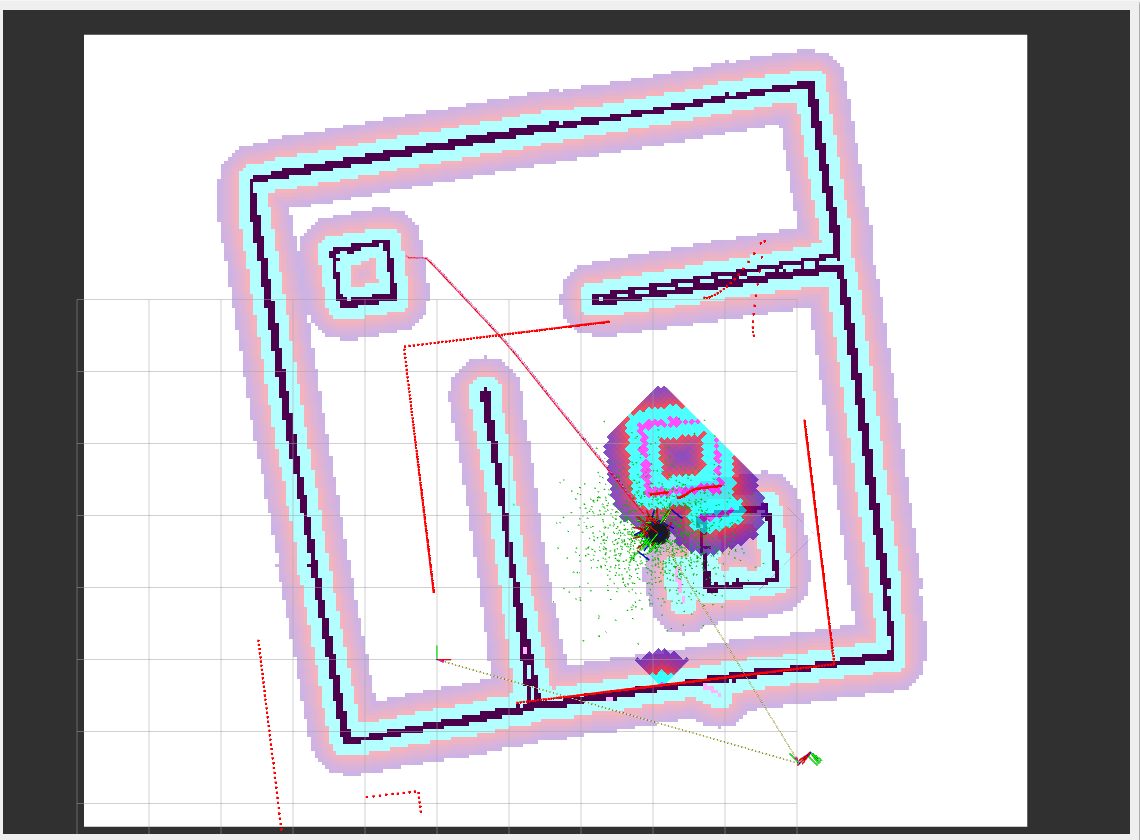
\includegraphics[width=\linewidth]{fig_amcl_before.png}\caption{initial pose với $\sigma_{xy}=0{,}5$\,m, $\sigma_\theta=0{,}4$\,rad: hạt (chấm xanh lá) rải rộng.}\end{subfigure}\hfill
\begin{subfigure}{0.49\linewidth}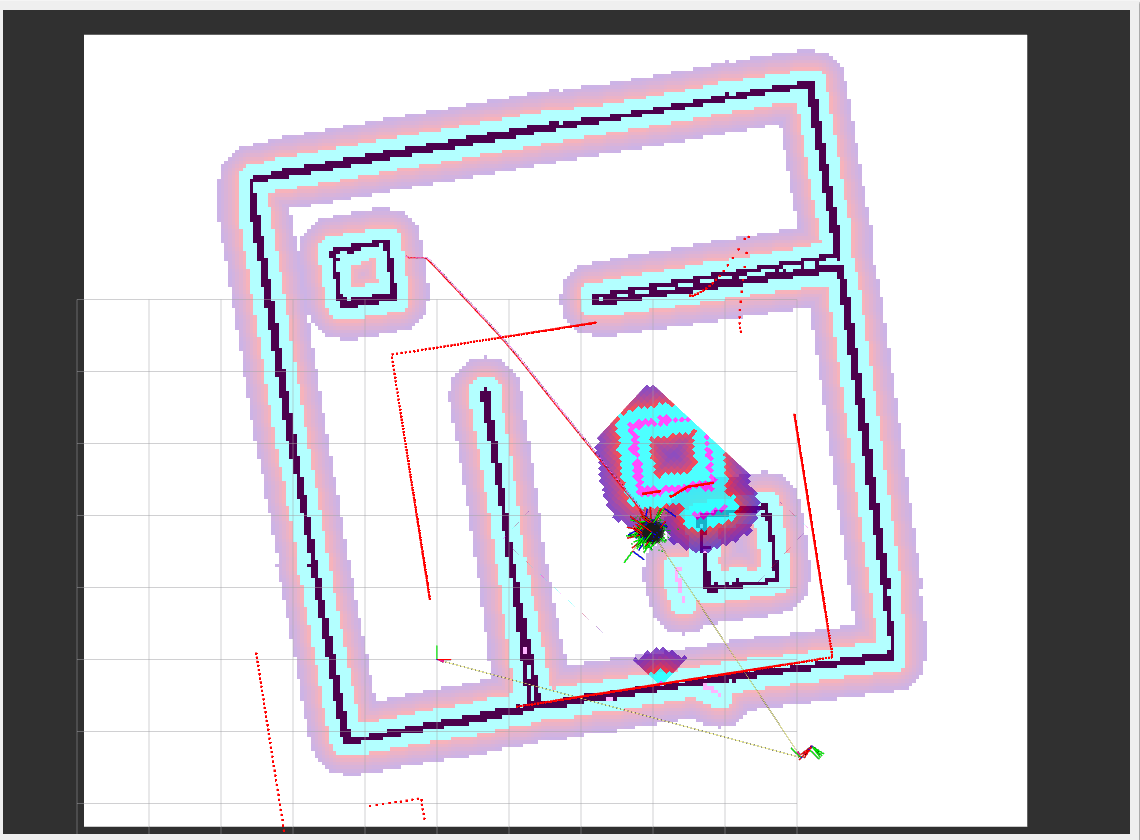
\includegraphics[width=\linewidth]{fig_amcl_after.png}\caption{với $\sigma_{xy}=0{,}1$\,m, $\sigma_\theta=0{,}1$\,rad: hạt tụ gọn quanh robot; AMCL báo $\sigma\approx0{,}10$\,m, $5{,}4^\circ$.}\end{subfigure}
\caption{Đám hạt AMCL trong RViz2 (vùng màu quanh robot là local costmap; tia LiDAR đỏ trùng tường bản đồ).}\end{figure}

\section{Phần 4 -- Navigation với Nav2}

\subsection{Khởi chạy}
Nav2 chạy \emph{sau} localization (AMCL cung cấp TF \code{map}$\to$\code{odom} và \code{map\_server} cung cấp \code{/map}) và sau khi đã đặt initial pose:
\begin{lstlisting}[language=bash,caption={\file{scripts/start\_nav2.sh}.}]
exec ros2 launch turtlebot4_navigation nav2.launch.py use_sim_time:=true \
  params_file:="$DIR/config/nav2.yaml" "$@"
\end{lstlisting}
Launch này gọi \code{nav2\_bringup/navigation\_launch.py}, đặt lại tên \code{cmd\_vel}: controller phát \code{cmd\_vel\_nav}, \code{velocity\_smoother}
làm mượt rồi phát \code{cmd\_vel} (topic mà \code{motion\_control} của robot nhận). Log xác nhận các node đã \emph{active}:
\begin{lstlisting}[numbers=none,basicstyle=\ttfamily\footnotesize,caption={Cuối log \code{start\_nav2.sh}.}]
[lifecycle_manager_navigation]: Server velocity_smoother connected with bond.
[lifecycle_manager_navigation]: Managed nodes are active
\end{lstlisting}

\subsection{Nav2 lập kế hoạch và điều khiển như thế nào}
\begin{figure}[H]\centering
\small
\begin{tabular}{c}
Goal (RViz2 \emph{Nav2 Goal} $\rightarrow$ action \code{navigate\_to\_pose})\\
$\downarrow$\\
\textbf{bt\_navigator} (cây hành vi: lập kế hoạch lại $+$ phục hồi)\\
$\downarrow$ \code{compute\_path\_to\_pose}\hspace{2cm}$\downarrow$ \code{follow\_path}\\
\textbf{planner\_server} (NavFn) \hspace{1cm}$\rightarrow$ \code{/plan} $\rightarrow$\hspace{1cm} \textbf{controller\_server} (DWB)\\
dùng \textbf{global\_costmap}\hspace{4.2cm}dùng \textbf{local\_costmap}\\
$\downarrow$\\
\code{/cmd\_vel\_nav} $\rightarrow$ \textbf{velocity\_smoother} $\rightarrow$ \code{/cmd\_vel} $\rightarrow$ \code{motion\_control} $\rightarrow$ bánh xe\\
\end{tabular}
\caption{Luồng dữ liệu của Nav2 trong bài.}
\end{figure}

\paragraph{Bản đồ chi phí (costmap).} \code{global\_costmap} (frame \code{map}, cập nhật 1\,Hz) gồm \code{static\_layer} (từ \code{/map}),
\code{obstacle\_layer} (từ \code{/scan}) và \code{inflation\_layer}. \code{local\_costmap} (frame \code{odom}, cửa sổ trượt $3\times 3$\,m, 5\,Hz) dùng
\code{voxel\_layer}. \code{inflation\_layer} làm phồng vật cản: các ô trong bán kính \code{inflation\_radius} quanh tường có chi phí giảm dần
theo $\exp(-\text{cost\_scaling\_factor}\cdot(d-r_{\text{robot}}))$, nên đường đi tránh sát tường.
\begin{lstlisting}[language=yaml,caption={Trích \file{config/nav2.yaml}: costmap.}]
robot_radius: 0.175
inflation_layer:
  plugin: "nav2_costmap_2d::InflationLayer"
  cost_scaling_factor: 4.0
  inflation_radius: 0.45
obstacle_layer / voxel_layer:
  observation_sources: scan
  raytrace_max_range: 3.0
  obstacle_max_range: 2.5
\end{lstlisting}

\paragraph{Lập kế hoạch toàn cục (planner\_server).} Dùng \code{nav2\_navfn\_planner/NavfnPlanner} (Dijkstra, \code{use\_astar: false}) trên \code{global\_costmap};
\code{tolerance: 0.5} cho phép goal lệch tối đa 0,5\,m nếu ô goal không đi được. Kết quả là đường đi ngắn nhất tránh vùng chi phí cao, phát trên \code{/plan}.
\begin{lstlisting}[language=yaml,caption={Trích \file{config/nav2.yaml}: planner.}]
planner_server:
  ros__parameters:
    expected_planner_frequency: 20.0
    planner_plugins: ["GridBased"]
    GridBased:
      plugin: "nav2_navfn_planner/NavfnPlanner"
      tolerance: 0.5
      use_astar: false
\end{lstlisting}

\paragraph{Điều khiển cục bộ (controller\_server).} Chạy ở 20\,Hz với \code{dwb\_core::DWBLocalPlanner} (Dynamic Window Approach). Mỗi chu kỳ DWB lấy mẫu
các cặp $(v,\omega)$ khả dĩ trong cửa sổ động (giới hạn tốc độ và gia tốc), mô phỏng quỹ đạo \code{sim\_time}=1,7\,s về phía trước trên \code{local\_costmap},
chấm điểm từng quỹ đạo bằng các \emph{critic} và chọn quỹ đạo điểm tốt nhất: \code{BaseObstacle} (tránh vật cản), \code{PathAlign}/\code{PathDist}
(bám đường toàn cục), \code{GoalAlign}/\code{GoalDist} (tiến gần goal), \code{RotateToGoal} (xoay đúng hướng ở đích), \code{Oscillation} (chống dao động).
\begin{lstlisting}[language=yaml,caption={Trích \file{config/nav2.yaml}: controller.}]
controller_server:
  ros__parameters:
    controller_frequency: 20.0
    general_goal_checker:
      plugin: "nav2_controller::SimpleGoalChecker"
      xy_goal_tolerance: 0.25
      yaw_goal_tolerance: 0.25
    FollowPath:
      plugin: "dwb_core::DWBLocalPlanner"
      max_vel_x: 0.26      max_vel_theta: 1.0
      acc_lim_x: 2.5       acc_lim_theta: 3.2
      vx_samples: 20       sim_time: 1.7
      critics: ["RotateToGoal", "Oscillation", "BaseObstacle", "GoalAlign",
                "PathAlign", "PathDist", "GoalDist"]
\end{lstlisting}

\paragraph{Cây hành vi và phục hồi (bt\_navigator, behavior\_server).} Mặc định dùng cây
\code{navigate\_to\_pose\_w\_\allowbreak replanning\_and\_\allowbreak recovery}: lập kế hoạch lại định kỳ, theo đường đi; nếu thất bại thì xóa costmap và chạy các hành vi phục hồi
của \code{behavior\_server} (\code{spin}, \code{backup}, \code{wait}, ...) rồi thử lại. Goal chỉ ``thành công'' khi robot vào trong
\code{xy\_goal\_tolerance}=0,25\,m (và đúng hướng trong 0,25\,rad).

\paragraph{Làm mượt vận tốc.} \code{velocity\_smoother} giới hạn tốc độ $\pm0{,}26$\,m/s, $\pm1{,}0$\,rad/s và gia tốc $2{,}5$\,m/s$^2$, $3{,}2$\,rad/s$^2$ trước khi gửi \code{/cmd\_vel}.

\subsection{Thực hiện navigation goal}
Sau khi AMCL đã hội tụ (Phần 3), em đặt goal. Trong video demo, goal được đặt bằng công cụ \emph{Nav2 Goal} của RViz2 (không lái tay sau đó).
Để có số liệu có thể kiểm chứng (thời gian, quãng đường, khoảng cách tối thiểu tới tường), em còn dùng \file{scripts/send\_goals.py}, gửi cùng loại goal
\code{NavigateToPose} qua action server và ghi lại vị trí AMCL và khoảng cách nhỏ nhất của \code{/scan}:
\begin{lstlisting}[language=Python,caption={Trích \file{scripts/send\_goals.py}.}]
client = ActionClient(node, NavigateToPose, 'navigate_to_pose')
msg = NavigateToPose.Goal()
msg.pose.header.frame_id = 'map'
msg.pose.pose.position.x, msg.pose.pose.position.y = gx, gy
msg.pose.pose.orientation.z, msg.pose.pose.orientation.w = math.sin(gyaw/2), math.cos(gyaw/2)
fut = client.send_goal_async(msg)
\end{lstlisting}
Bốn goal ở bốn khu vực khác nhau của bản đồ (tọa độ trong frame \code{map}):
\begin{table}[H]\centering\small
\begin{tabular}{clcccc}\toprule
Goal & Khu vực & Tọa độ & Kết quả & Quãng đường & Cách tường gần nhất\\\midrule
1 & phải-giữa, gần hộp & (3,0; 2,0) & thành công (lần 2) & 1,62\,m & 0,37\,m\\
2 & hành lang phía bắc & (2,5; 5,6) & thành công & 7,41\,m & 0,46\,m\\
3 & góc tây-bắc, cạnh hộp & ($-0{,}4$; 5,6) & thành công & 2,60\,m & 0,48\,m\\
4 & đông-nam & (3,5; 0,2) & thành công & 6,73\,m & 0,41\,m\\
\bottomrule\end{tabular}
\caption{Kết quả bốn goal (nguồn: \file{logs/04\_nav\_goals.log}, \file{logs/05\_nav\_goal1\_retry.log}). Sai số tới đích đo bằng \code{/amcl\_pose} sau khi goal kết thúc: 0,21; 0,20; 0,28; 0,19\,m (goal 1--4). Goal checker xác nhận ``thành công'' với ngưỡng 0,25\,m; số 0,28\,m của goal 3 hơi lớn hơn ngưỡng. Em chưa xác định chắc lý do; có thể do \code{/amcl\_pose} chỉ cập nhật khi robot đi đủ \code{update\_min\_d}=0,25\,m nên giá trị em đọc có thể cũ, hoặc do sai số định vị AMCL, nên không nên coi con số này chính xác hơn vài cm.}\label{tab:goals}
\end{table}
\paragraph{Về goal 1.} Lần đầu goal 1 bị \emph{ABORTED}: planner báo
\emph{``Planning algorithm GridBased failed to generate a valid path to (3.00, 2.00)''}, robot chỉ đi 0,85\,m.
Đến khi chạy lại goal này (sau goal 2--4) thì thành công trong 39\,s. Em chưa xác định chắc nguyên nhân thất bại lần đầu; thời điểm đó
AMCL vừa hội tụ và robot ở gần vị trí xuất phát, nên có thể do costmap/định vị chưa ổn định hoặc robot đứng trong vùng phồng của vách. Vì thế 3 goal liên tiếp đầu tiên
đạt yêu cầu là goal 2, 3, 4; goal 1 thành công ở lần thử lại.

\paragraph{Va chạm.} Khoảng cách nhỏ nhất từ LiDAR tới vật cản trong cả hành trình là 0,37--0,48\,m (robot bán kính 0,175\,m), tức không sát hay chạm tường.
Số liệu này lấy từ \code{/scan} nên chỉ phản ánh vật cản trong mặt phẳng LiDAR. Log của \code{motion\_control} chỉ có các dòng bật reflex lúc khởi động
(\emph{Enabling REFLEX\_BUMP/CLIFF/STUCK/WHEEL\_DROP}), không có sự kiện hazard hay reflex nào trong lúc chạy Nav2; em không ghi riêng topic \code{/hazard\_detection}. Quỹ đạo thật vẽ ở hình dưới.
\begin{figure}[tbp]\centering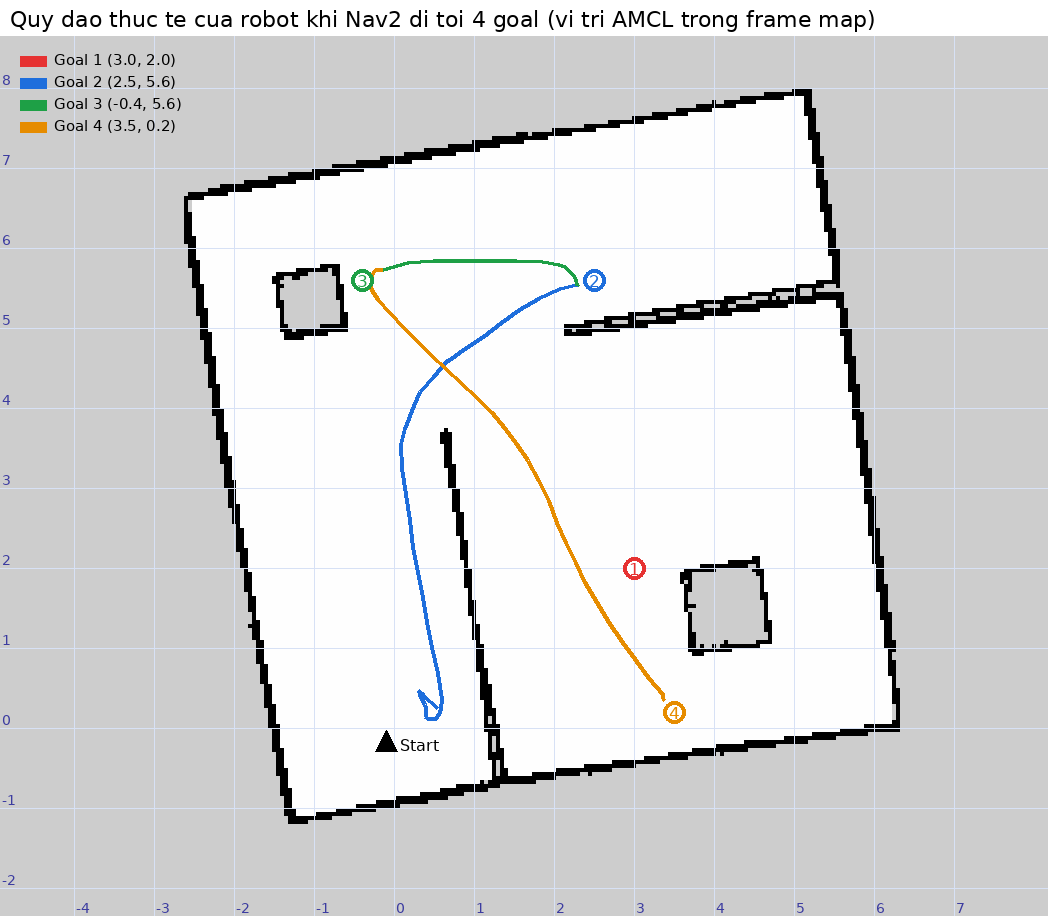
\includegraphics[width=0.9\linewidth]{fig_nav_trajectory.png}
\caption{Quỹ đạo robot (vị trí AMCL) khi Nav2 đi đến goal 2, 3, 4, vẽ trên bản đồ từ \file{logs/nav\_trajectory\_run1.csv}. Số trong vòng tròn là vị trí goal, tam giác đen là vị trí xuất phát. Quỹ đạo của lần chạy lại goal 1 không vẽ được vì file CSV của lần đó đã bị lần gửi goal thứ 5 ghi đè (script lúc đó luôn ghi cùng tên file); chỉ còn số liệu tổng hợp trong \file{logs/05\_nav\_goal1\_retry.log}.}\end{figure}
\begin{figure}[tbp]\centering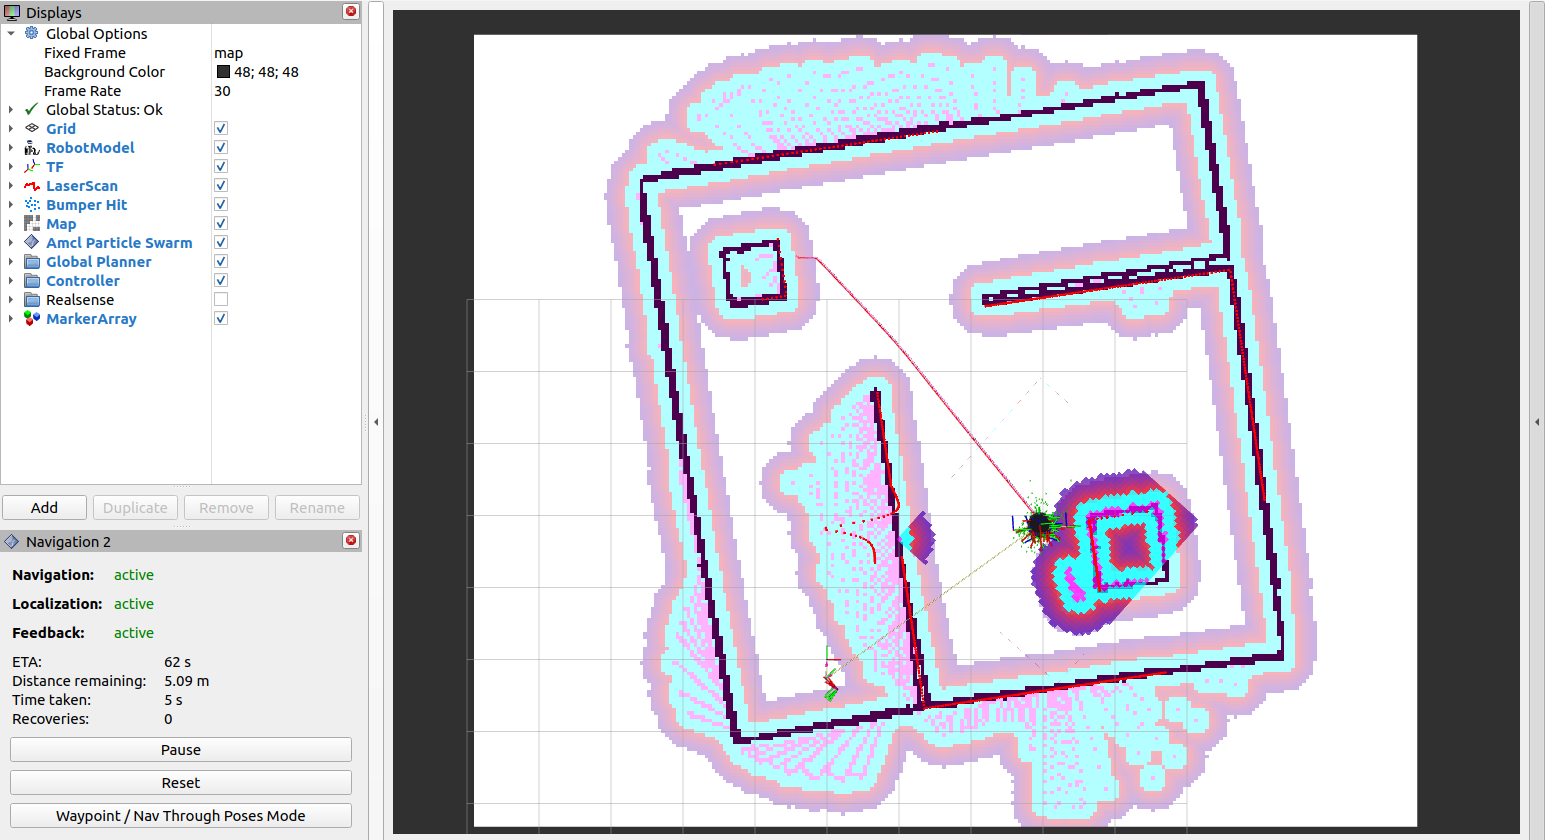
\includegraphics[width=\linewidth]{fig_nav_goal.png}
\caption{RViz2 khi Nav2 đang thực hiện một goal: global costmap (vùng màu quanh tường là inflation), local costmap (ô vuông quanh robot), đường đi toàn cục màu đỏ từ robot tới goal ở góc tây-bắc, hạt AMCL màu xanh lá; bảng \emph{Navigation 2} bên trái báo Navigation/Localization: active. Ảnh chụp ở lần gửi goal thứ 5 (xem mục \ref{sec:goal5}).}\label{fig:navgoal}\end{figure}

\paragraph{Lần gửi goal thứ 5 (thất bại).}\label{sec:goal5} Để chụp Hình~\ref{fig:navgoal}, sau khi hệ thống đã chạy liên tục hơn 2\,200\,s giờ mô phỏng, em gửi lại goal $(-0{,}4;\,5{,}6)$. Planner vẫn tạo được đường đi (Hình~\ref{fig:navgoal}) nhưng robot không tiến được: \code{controller\_server} liên tục báo \emph{``Transform data too old when converting from map to odom''} (TF \code{map}$\to$\code{odom} mà nó giữ có mốc thời gian 1\,235\,s trong khi dữ liệu là 2\,247\,s), rồi \emph{``Failed to make progress''}; hành vi phục hồi \code{spin} cũng thất bại vì \emph{``Current footprint not available''}. Script hủy goal sau 600\,s; robot chỉ dao động quanh chỗ cũ (quãng đường tích lũy 10,4\,m nhưng vị trí thay đổi dưới 0,25\,m) và không va chạm (cách tường $\ge 0{,}50$\,m). Em chưa xác định được nguyên nhân gốc; nghi là bộ đệm TF của Nav2 bị lệch sau một lần RViz2 bị tắt và mở lại, kết hợp máy quá tải (load average 48--60). Vì vậy số liệu chính thức của Phần~4 là 4 goal ở Bảng~\ref{tab:goals}; lần thứ 5 được ghi lại để trung thực (\file{logs/07\_nav\_goal\_rviz\_shot.log}).

\section{Node, topic chính và trả lời câu hỏi}

\subsection{Các node chính khi Nav2 đang chạy}
Danh sách thu từ \code{ros2 node list} (\file{logs/06\_system\_info.log}), lọc các node liên quan:
\begin{table}[H]\centering\small
\begin{tabular}{p{4.6cm}p{10cm}}\toprule
\textbf{Node} & \textbf{Chức năng}\\\midrule
\code{/lidar\_bridge} & Cầu nối Gazebo $\to$ ROS cho \code{/scan}\\
\code{/diffdrive\_controller} & Điều khiển bánh vi sai, phát \code{/odom} và TF \code{odom}$\to$\code{base\_link}\\
\code{/motion\_control} & Create~3: nhận \code{/cmd\_vel}, áp dụng an toàn (reflex, \code{safety\_override})\\
\code{/robot\_state\_publisher} & Phát TF tĩnh từ URDF (\code{base\_link}$\to$\code{rplidar\_link}, ...)\\
\code{/map\_server} & Nạp \code{map.yaml}, phát \code{/map}\\
\code{/amcl} & Định vị, nhận \code{/scan}, \code{/odom}, \code{/initialpose}; phát \code{/amcl\_pose}, \code{/particle\_cloud}, TF \code{map}$\to$\code{odom}\\
\code{/bt\_navigator} & Máy chủ action \code{navigate\_to\_pose}; chạy cây hành vi\\
\code{/planner\_server} & Lập kế hoạch toàn cục (NavFn), action \code{compute\_path\_to\_pose}\\
\code{/controller\_server} & Điều khiển cục bộ (DWB), action \code{follow\_path}\\
\code{/global\_costmap}, \code{/local\_costmap} & Hai bản đồ chi phí\\
\code{/behavior\_server} & Hành vi phục hồi: \code{spin}, \code{backup}, \code{wait}\\
\code{/smoother\_server}, \code{/velocity\_smoother} & Làm mượt đường đi và vận tốc\\
\code{/lifecycle\_manager\_*} & Khởi động/giám sát các node vòng đời (lifecycle)\\
\bottomrule\end{tabular}
\caption{Node chính.}
\end{table}

\subsection{Các topic chính}
\begin{table}[H]\centering\small
\begin{tabular}{lll}\toprule
\textbf{Topic} & \textbf{Kiểu} & \textbf{Ghi chú}\\\midrule
\code{/scan} & \code{sensor\_msgs/LaserScan} & LiDAR, SLAM/AMCL/costmap đều dùng\\
\code{/odom} & \code{nav\_msgs/Odometry} & odometry bánh xe\\
\code{/cmd\_vel} & \code{geometry\_msgs/Twist} & lệnh vận tốc tới robot\\
\code{/cmd\_vel\_nav} & \code{geometry\_msgs/Twist} & đầu ra controller, trước smoother\\
\code{/tf}, \code{/tf\_static} & \code{tf2\_msgs/TFMessage} & cây TF\\
\code{/clock} & \code{rosgraph\_msgs/Clock} & giờ mô phỏng\\
\code{/map} & \code{nav\_msgs/OccupancyGrid} & bản đồ (SLAM hoặc \code{map\_server})\\
\code{/initialpose} & \code{PoseWithCovarianceStamped} & vị trí ban đầu cho AMCL\\
\code{/amcl\_pose} & \code{PoseWithCovarianceStamped} & kết quả định vị\\
\code{/particle\_cloud} & \code{nav2\_msgs/ParticleCloud} & các hạt AMCL\\
\code{/goal\_pose} & \code{geometry\_msgs/PoseStamped} & goal từ RViz2\\
\code{/plan}, \code{/plan\_smoothed} & \code{nav\_msgs/Path} & đường đi toàn cục\\
\code{/global\_costmap/costmap}, \code{/local\_costmap/costmap} & \code{nav\_msgs/OccupancyGrid} & costmap\\
\bottomrule\end{tabular}
\caption{Topic chính.}
\end{table}
Số publisher của \code{/cmd\_vel} đo được là 7 vì nhiều node (teleop, smoother, bridge, ...) cùng có thể phát; chỉ \code{velocity\_smoother} phát khi Nav2 điều khiển.

\paragraph{Cây TF.} Chuỗi là \code{map} $\xrightarrow{\text{AMCL}}$ \code{odom} $\xrightarrow{\text{diffdrive}}$ \code{base\_link} $\xrightarrow{\text{URDF}}$ \code{rplidar\_link}.
\code{odom}$\to$\code{base\_link} liên tục nhưng trôi theo thời gian; \code{map}$\to$\code{odom} do AMCL (hoặc SLAM) bù để đưa về khung bản đồ cố định.
Ví dụ đo được: \code{tf2\_echo map base\_link} cho $(3{,}055;\,1{,}801)$, yaw $13{,}5^\circ$ khi robot đang ở gần goal 1.

\subsection{Trả lời các câu hỏi ``Nội dung cần hiểu''}
\emph{Ghi chú:} đề bài không kèm danh sách câu hỏi cụ thể trong bản em có, nên dưới đây là các câu hỏi cốt lõi về chủ đề bài;
nếu đề có câu khác, em sẽ bổ sung.

\paragraph{1. SLAM là gì, SLAM Toolbox làm gì?} SLAM (Simultaneous Localization and Mapping) là dựng bản đồ và ước lượng vị trí robot cùng lúc khi chưa biết trước cả hai.
SLAM Toolbox là SLAM 2D dựa trên đồ thị tư thế: mỗi scan là một nút, scan matching tạo ràng buộc giữa các nút kề nhau, loop closure tạo ràng buộc giữa các nút xa nhau khi quay lại chỗ cũ, rồi bộ giải (Ceres) tối ưu toàn đồ thị để giảm lệch tích lũy.

\paragraph{2. Vì sao cần cả \code{/odom} lẫn \code{/scan}?} \code{/odom} cho ước lượng chuyển động ngắn hạn, liên tục và mượt nhưng trôi (trượt bánh, sai số tích lũy). \code{/scan} đo khoảng cách tuyệt đối tới môi trường, dùng để sửa trôi qua scan matching. SLAM/AMCL lấy odometry làm giá trị dự đoán và dùng scan để hiệu chỉnh.

\paragraph{3. Bản đồ lưới chiếm dụng và hai file \code{map.pgm}, \code{map.yaml}.} \code{map.pgm} là ảnh xám: 0 (đen) là có vật cản, 254 (trắng) là trống, 205 là chưa biết. \code{map.yaml} là metadata: tên ảnh, \code{resolution} (m/điểm), \code{origin} (tọa độ góc dưới trái), ngưỡng \code{occupied\_thresh}/\code{free\_thresh}, \code{negate}.

\paragraph{4. Localization khác mapping thế nào? AMCL hoạt động ra sao?} Mapping dựng bản đồ chưa có; localization giữ bản đồ cố định và chỉ ước lượng vị trí robot trên đó.
AMCL (Adaptive Monte Carlo Localization) là bộ lọc hạt: giữ một tập hạt, mỗi hạt là một giả thuyết tư thế. Bước \emph{dự đoán} di chuyển các hạt theo odometry cộng nhiễu;
bước \emph{cập nhật} gán trọng số mỗi hạt theo mức scan hiện tại khớp bản đồ (mô hình \code{likelihood\_field}); bước \emph{lấy mẫu lại} giữ các hạt trọng số cao.
``Adaptive'' là số hạt tự thay đổi (500--2000) theo độ bất định. Khi hạt hội tụ, sigma nhỏ (đo được khoảng 0,15\,m và $8^\circ$).

\paragraph{5. Vì sao phải đặt initial pose?} Không có vị trí ban đầu, các hạt không biết bắt đầu ở đâu trên bản đồ; nhiều chỗ trong bản đồ trông giống nhau nên dễ hội tụ sai. Initial pose thu hẹp không gian tìm kiếm.
Khi em đặt sai, AMCL ở lại tư thế lệch (xem Phần~3); có thể dùng \code{/reinitialize\_global\_localization} để rải hạt khắp bản đồ, nhưng trong lần thử của em kết quả không đáng tin (sigma khoảng 1,7--3,0\,m và vị trí ước lượng lệch xa).

\paragraph{6. Vai trò các frame \code{map}, \code{odom}, \code{base\_link}?} \code{map}: khung cố định gắn với bản đồ; \code{odom}: khung liên tục nhưng trôi; \code{base\_link}: gắn với robot.
Nav2 lập kế hoạch trong \code{map}, điều khiển cục bộ trong \code{odom} (mượt, không nhảy khi AMCL hiệu chỉnh).

\paragraph{7. Nav2 lập kế hoạch và điều khiển thế nào?} Xem Phần~4: \code{planner\_server} (NavFn) tìm đường toàn cục trên global costmap; \code{controller\_server} (DWB) chọn $(v,\omega)$ bám đường đó và tránh vật cản bằng local costmap;
\code{bt\_navigator} điều phối và kích hoạt phục hồi khi kẹt; \code{velocity\_smoother} làm mượt lệnh trước khi gửi \code{/cmd\_vel}.

\paragraph{8. Costmap và inflation để làm gì?} Costmap biến bản đồ và dữ liệu cảm biến thành ``chi phí đi qua mỗi ô''. Inflation phồng vật cản bằng bán kính robot cộng biên an toàn, để chỉ cần coi robot là một điểm khi lập kế hoạch. Với \code{robot\_radius}=0,175\,m và \code{inflation\_radius}=0,45\,m, đường đi tránh sát tường (kết quả: cách tường $\ge 0{,}37$\,m).

\paragraph{9. Global planner và local planner khác nhau thế nào?} Global planner nhìn toàn bản đồ, ra đường đi dài hạn nhưng bỏ qua động học và vật cản mới. Local planner nhìn cửa sổ nhỏ, chạy tần số cao (20\,Hz), tính lệnh vận tốc cụ thể có xét giới hạn tốc độ/gia tốc và vật cản vừa quan sát.

\paragraph{10. Vì sao phải chạy với \code{use\_sim\_time:=true}?} Mọi node phải dùng \code{/clock} của Gazebo để mốc thời gian của TF, scan và odom khớp nhau; nếu lẫn giờ thật và giờ mô phỏng, TF báo ``extrapolation'' và các message bị loại.

\paragraph{11. Vì sao đặt \code{safety\_override} và undock?} Create~3 có cơ chế an toàn (hazard, reflex) và mặc định không cho robot chạy khi còn trên dock; \code{backup\_only} cho phép Nav2 chạy mà vẫn giữ an toàn khi lùi. Undock đưa robot ra khỏi trạm sạc.

\section{Kết luận, hạn chế và liên kết}

\subsection{Kết quả đạt được}
\begin{itemize}
\item Phần 1: robot chạy trong Gazebo; \code{/scan}, \code{/odom}, \code{/cmd\_vel} hoạt động (log \file{logs/01\_topic\_check.log}).
\item Phần 2: dựng và lưu bản đồ \file{maps/map.pgm}, \file{maps/map.yaml}; không có tường nhân đôi.
\item Phần 3: nạp bản đồ bằng \code{map\_server}, AMCL hội tụ (sigma khoảng 0,15\,m, $8^\circ$) sau khi đặt initial pose bằng khớp scan--bản đồ.
\item Phần 4: Nav2 đưa robot đến cả 4 goal ở các khu vực khác nhau mà không điều khiển tay; khoảng cách nhỏ nhất tới tường 0,37\,m.
\end{itemize}

\subsection{Hạn chế và những điều cần nói thẳng}
\begin{itemize}
\item \textbf{World tự tạo, nhỏ hơn} world \code{maze} có sẵn; \textbf{cảm biến bị giảm tần số} bằng URDF overlay, và cần \code{LIBGL\_ALWAYS\_SOFTWARE=1}. Đề cho phép dùng môi trường có sẵn nhưng không cấm môi trường tự tạo; lý do là hiệu năng máy.
\item \textbf{Bản đồ có hậu xử lý} bằng \code{clean\_map.py} (xóa điểm lẻ bên ngoài tường); bản thô được giữ lại trong \file{maps/map\_raw.pgm}.
\item \textbf{Bản đồ được quét bằng lái tay}, đúng yêu cầu đề; node tự động bám tường em viết thử không dùng.
\item \textbf{Initial pose lấy từ khớp scan--bản đồ}, nên số liệu ``AMCL trùng với khớp scan'' không phải kiểm chứng độc lập; chưa có vị trí thật từ Gazebo để so (topic ground truth lỗi QoS). Kiểm chứng định tính là tia LiDAR trùng tường và robot tới đúng các goal.
\item \textbf{Goal 1 thất bại lần đầu} (planner không tạo được đường), thành công khi thử lại; chưa xác định chắc nguyên nhân.
\item Số liệu goal ghi bằng script \code{send\_goals.py} (cùng action \code{NavigateToPose}); phần đặt goal bằng công cụ Nav2 Goal của RViz2 được thể hiện trong video/ảnh.
\item Lần gửi goal thứ 5 (để chụp ảnh) thất bại với lỗi TF \emph{Transform data too old} sau khi hệ thống chạy lâu; nguyên nhân gốc chưa rõ (mục~\ref{sec:goal5}).
\item Khi Wi-Fi rớt, Gazebo Transport (multicast) mất kết nối làm \code{/odom}, \code{/scan} ngừng; cần chạy lại mô phỏng. Đây là lỗi môi trường, không phải lỗi thuật toán.
\end{itemize}

\subsection{Liên kết}
\begin{itemize}
\item Video demo (Google Drive, công khai): \texttt{[LINK-VIDEO-GOOGLE-DRIVE]}
\item GitHub repository (Public): \texttt{https://github.com/[GITHUB-USER]/[TÊN-REPO]}
\end{itemize}

\subsection{Tài liệu tham khảo}
\begin{itemize}
\item TurtleBot~4 Simulator: \url{https://github.com/turtlebot/turtlebot4_simulator}
\item TurtleBot~4 User Manual: \url{https://turtlebot.github.io/turtlebot4-user-manual/}
\item SLAM Toolbox: \url{https://github.com/SteveMacenski/slam_toolbox}; Nav2: \url{https://docs.nav2.org}
\end{itemize}

\end{document}
